% !TEX root = CSL 2021.tex

%\subparagraph*{Measuring sensitivity and similarity of programs in a compositional way}
In program semantics one is usually interested in capturing notions of behavioral equivalence between programs. However,  sin several fields like approximate \cite{Mittal2016}, incremental \cite{Cai2014, Picallo2019} and probabilistic \cite{10.1109/LICS.2015.64} computation, it is often more useful to be able to describe \emph{to which extent}  two programs behave in a similar, although non equivalent way, so that one can measure the change in the result produced by
replacing one program by the other one.
% produces a change in the result which can be quantified and bounded in some way.



This idea has motivated much literature on program (pseudo)metrics \cite{ARNOLD1980181, VANBREUGEL20011,Azevedo_de_Amorim_2017, Escardo1999, BAIER1994171,10.1109/LICS.2015.64, 10.1007/978-3-662-44584-6_4, 10.1007/978-3-662-54434-1_13, 10.1145/3209108.3209149}, that is, on semantics in which types are endowed with a notion of distance measuring the differences in their behaviors. This approach has found widespread applications, for example in differential privacy \cite{10.1145/1932681.1863568, 10.1007/978-3-642-29420-4_3, Barthe_2012}, where one is interested in measuring the \emph{sensitivity} of a program, \textit{i.e.} its capacity to amplify changes in its inputs, and in the study of probabilistic processes \cite{DESHARNAIS2004323, VANBREUGEL2005115, 10.1007/978-3-662-44584-6_4,10.1007/3-540-48224-5_35}.


Recent literature \cite{chaudhuri, dallago:differential-stlc} has highlighted the importance of \emph{contextuality} to reason about program similarity: many common situations  require to measure the error produced by a transformation of the form $\mathtt C[t] \leadsto \mathtt C[u]$, which replaces a program $t$ by $u$ \emph{within a context} $\mathtt C[\ ]$, as a function of the mismatch between $t$ and $u$ and of the sensitivity of the context $\mathtt C[\ ]$ itself.
 For instance, the error produced by replacing the program $\lambda x.\sin(x)$ by the identity function $\lambda x.x$
  in a given context  $\mathtt C$ will 
  be highly sensitive to how close to $0$  
  these functions are evaluated in $\mathtt C$.
 Similar cases of contextual reasoning can be found  in many areas of computer science: for example 
 in techniques from numerical analysis (\emph{e.g.}~the Gauss-Newton method), in which a 
 computationally intensive function is replaced by its Taylor's expansion {around some given point}, or in {approximate computing} techniques like \emph{loop perforation} \cite{loopperf}, in which a compiler can be asked to skip a certain number of iterations of a loop in a program.

\subparagraph*{The Problem of Coupling Program Metrics with Higher-Order Types}

\begin{figure}
\begin{subfigure}{0.48\textwidth}
\parbox[h][3.5cm][c]{\textwidth}{
\adjustbox{center}{$
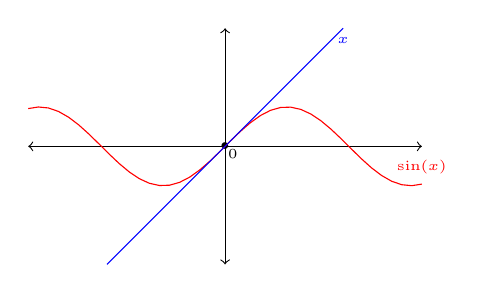
\begin{tikzpicture}[domain=-5:5, scale=0.5]
%\draw[very thin,color=gray] (-0.1,-1.1) grid (3.9,3.9);
\draw[<->]   (-5,0) -- (5,0);
\draw[<->] (0,-3) -- (0,3); % node[above] {$f(x)$};

   \node at (0.2,-0.2){\tiny$0$};
      \node at (0,0){\tiny$\bullet$};

%
\draw[color=red, domain=-5:5, samples=40] plot (\x, {sin(\x r)} ) node[above] {\tiny$\sin(x)$};

\draw[color=blue, domain=-3:3, samples=40] plot (\x,{\x  } ) node[below] {\tiny$x$};


\end{tikzpicture}$}
}
\caption{\small $\sin(x)$ and $x$ are very close around $0$, but their distance diverges at $\pm \infty$.}
\label{fig:sinid1}
\end{subfigure} \ \ \ 
\begin{subfigure}{0.48\textwidth}
\parbox[h][3.5cm][c]{\textwidth}{
\adjustbox{center}{$
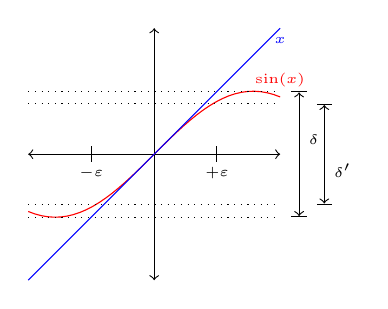
\begin{tikzpicture}[domain=-2:2, scale=0.8]
%\draw[very thin,color=gray] (-0.1,-1.1) grid (3.9,3.9);
\draw[<->]   (-2,0) -- (2,0);
\draw[<->] (0,-2) -- (0,2); % node[above] {$f(x)$};


\draw[|-|] (-1,0) -- (1,0);
\node(r) at (-1,-0.3) {\tiny$-\varepsilon$};
\node(r) at (1,-0.3) {\tiny$+\varepsilon$};
   % \node at (0,0)[circle,fill,inner sep=1pt]{};
%
\draw[color=red, domain=-2:2, samples=40] plot (\x, {sin(\x r) } ) node[above] {\tiny$\sin(x)$};

\draw[color=blue, domain=-2:2,samples=40] plot (\x,{\x  } ) node[below] {\tiny$x$};


\draw[dotted] (-2,1) -- (2,1);
\draw[dotted] (-2,-1) -- (2,-1);

\draw[dotted] (-2,0.8) -- (2,0.8);
\draw[dotted] (-2,-0.8) -- (2,-0.8);

\draw[|<->|] (2.3,1) -- node[above right]{\tiny$\delta$} (2.3,-1);
\draw[|<->|] (2.7,0.8) -- node[below right]{\tiny$\delta'$} (2.7,-0.8);


\end{tikzpicture}$}
}
\caption{\small The self-distances $\delta,\delta'$ of $\sin(x)$ and $x$ in a small interval $[-\varepsilon,\varepsilon]$ of $0$ are very close.}
\label{fig:sinid2}
\end{subfigure}
\caption{The sup-distance is inadequate for contextual transformations.}
\label{fig:sinid}
\end{figure}
 
While several frameworks  for contextual reasoning have been developed in recent years \cite{10.1145/1932681.1863568,Gaboardi_2013,Azevedo_de_Amorim_2017,chaudhuri, dallago:differential-stlc}, these approaches suggest that describing program similarity for a fully higher-order language in terms of program metrics still constitutes a major challenge. 

In particular, when considering higher-order languages with a type $\mathsf{Real}$ for real numbers, it is not clear how to \emph{lift} the standard metric on $\mathsf{Real}$  
 to higher-order types, \emph{e.g.}~to $\mathsf{Real}\to \mathsf{Real}$, so that the distances between higher-order programs are measured in a contextual way.



A standard solution is to take the sup-distance, that is, to let, for $f,g:\mathsf{Real}\to \mathsf{Real}$, $d(f,g)=\sup\{d(f(r),g(r))\mid r\in \mathsf{Real}\}$. This solution works well in models in which programs are interpreted as \emph{non-expansive} or \emph{Lipschitz-continuous} maps \cite{Hofmann2014, Azevedo_de_Amorim_2017}. However such models are not \emph{cartesian-closed}\footnote{In fact, cartesian closed categories of metric spaces and non-expansive functions \emph{do} exist \cite{Escardo1999, Stubbe2009}, but, to our knowledge, none of these categories contains the real numbers with the standard metric.}, so they do not account for 
 the simply-typed lambda-calculus in its full generality, but only for linear or sub-exponential variations of it (such as $\mathsf{Fuzz}$ \cite{10.1145/1932681.1863568,Gaboardi_2013,Azevedo_de_Amorim_2017}).
 Also, it has been shown \cite{10.1109/LICS.2015.64} that in a probabilistic setting the non-linearity of higher-order programs has the effect of \emph{trivialising} metrics, that is, of forcing distances to be either $0$ or $1$, hence collapsing program distances onto usual notions of program equivalence.
Most importantly, even if one restricts to a sub-exponential language, the sup-distance is inadequate to account for contextual transformations as the replacement of $\lambda x.\sin(x)$ by $\lambda x.x$ around $0$, as the sup-distance between these two programs is infinite (see Fig. \ref{fig:sinid}). 
 
 
On the other side of the coin, other approaches like \cite{chaudhuri, dallago:differential-stlc} are fully contextual and higher-order, but provide, at best, only weak approximations of a standard notion of metric.  
 Nonetheless, these approaches introduce the idea, which we retain here, that program differences must be taken as being themselves some kind of programs, relating errors in input with errors in  output, and that accordingly, programs should be split in two different classes: \emph{exact} programs, computing mappings from well-defined inputs to well-defined outputs, and \emph{approximate} programs, mapping errors in the input to errors in the output.


\subparagraph*{Diameter Spaces}

In this paper we introduce a new semantic framework to reason about program similarity and approximate program transformations based on 
a class of higher-order denotational models that we call \emph{diameter space models}. Compared to existing higher-order frameworks, the main novelty of these models is that program similarities are measured by associating each simple type with 
 a \emph{generalized partial metric space}, yielding a lifting of the standard metric on $\mathsf{Real}$ to higher-order types.

Generalized partial metric spaces are a well-investigated class of metric spaces that has been widely applied in program semantics \cite{bkmp:partial-metrics, Bukatin1997, doi:10.1111/j.1749-6632.1994.tb44144.x, Schellekens2004, Samet:2013aa, Stubbe2018, HE201999}. 
Such spaces generalize standard metric spaces in that distances
need not be real numbers, but can be functions or any other type of object that lives in a suitable \emph{quantale} \cite{Hofmann2014}, and \emph{self-distances} $d(x,x)$ need not be $0$ (which leads to a stronger triangular inequality: $d(x,y) + d(z,z)\leq d(x,z)+d(z,y)$).


In our models a higher-order type $A$ is interpreted as a 4-tuple $(|A|, \intervals{A}, \distances{A}, \diam_{A})$ called a \emph{diameter space}, where $|A|$ is a set of \emph{exact} values, $\intervals{A}\subset \mathcal P(|A|)$ is a complete lattice of \emph{approximate} values, $\distances{A}$ is a {quantale}, and $\diam_{A}: \intervals{A}\to \distances{A}$ is a function, called \emph{diameter}, which provides a quantitative measure of approximate values.
The map $\diam_{A}$ generalizes some properties of the diameter function of the standard metric on real numbers. In particular, just like the distance between two real numbers can be described as the diameter of the smallest interval containing them, the map $\diam_{A}$ yields a generalized partial metric  $d_{A}:|A|\times |A|\to \distances{A}$ in which the distance between two exact values of $A$ is measured as the diameter of the smallest approximate value containing them, i.e.  $d_{A}(x,y)=\diam_{A}(x\vee y)$. 


\subparagraph*{New Ways of Measuring Distances between Programs of Functional Type}
% measure distances on $\mathsf{Real}\to\mathsf{Real}$}\varepsilon

In our model, while the distance between two real numbers is measured with the standard metrics (and thus lives in the quantale $[0,\infty]$), the distance between  two programs $f,g:\mathsf{Real}\to \mathsf{Real}$ lives in the functional quantale of monotone maps from \emph{approximate values} of $\mathsf{Real}$ (\emph{i.e.} closed intervals) to positive reals. This function maps a closed interval $a$ to the diameter of the smallest interval containing \emph{both} $f(a)$ and $g(a)$. 
Note that, with this definition, 
 the distance of $f$ \emph{from itself}, which needs not be (constantly) 0,  provides a measure of the sensitivity of $f$, since it associates each interval $a$ with the size of the interval $f(a)$ spanned by $f$ on $a$. 
 

The use of partial metrics with functional distances yields a rich and expressive framework to reason about  
contextual transformations. For instance, we can express the closeness of $\lambda x.\sin(x)$ and $\lambda x.x$ around 0 by the fact that their distance, applied to a small interval $[-\varepsilon,\varepsilon]$ around 0, is very close to the {self-distance} of
$\lambda x.\sin(x)$ on the same interval (as illustrated in Fig. \ref{fig:sinid2}). Moreover, the {triangular inequality} of partial metrics  can be used to infer new bounds from previously established ones in a compositional way.


\begin{figure}
\begin{subfigure}{0.45\textwidth}
\parbox[h][4.6cm][c]{\textwidth}{
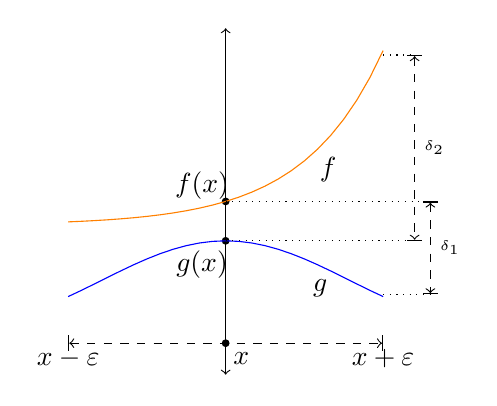
\begin{tikzpicture}[domain=-2:2]
%\draw[very thin,color=gray] (-0.1,-1.1) grid (3.9,3.9);
\draw[dashed, |<->|]   (-2,0) -- (2,0);
\draw[<->] (0,-0.4) -- (0,4); % node[above] {$f(x)$};

    \node at (0,0)[circle,fill,inner sep=1pt]{};
%    \node at (-2,0)[circle,fill,inner sep=1pt]{};
%    \node at (2,0)[circle,fill,inner sep=1pt]{};
\node(z) at (0.2,-0.2) {$x$};
\node(-e) at (-2,-0.2) {$x-\varepsilon$};
\node(e) at (2,-0.2) {$x+\varepsilon$};


\node(f) at (0,0.8+0.5)[circle,fill,inner sep=1pt]{};
\node(f) at (0,1.5+0.3)[circle,fill,inner sep=1pt]{};

\node(f) at (-0.3,2) {$f(x)$};

\node(f) at (-0.3,1) {$g(x)$};


\node(ff) at (1.3,2.2) {{$f$}};
\node(gg) at (1.2,0.7) {{$g$}};

%\draw[color=red] plot (\x,\x) node[right] {$f(x) =x$};
% \x r means to convert ?\x? from degrees to _r_adians:
\draw[color=blue] plot (\x,{0.8+ 0.5*(cos(\x r))}) ;
\draw[color=orange] plot (\x,{1.5+0.3*exp(\x)}) ;

\draw[dotted] (0,1.8) -- (2.6,1.8);
\draw[dotted] (2,0.62) -- (2.6,0.62);
\draw[dotted] (0,1.3) -- (2.4,1.3);
\draw[dotted] (2,3.66) -- (2.4,3.66);

%
%\draw[dotted] (0,1.8) -- (2, 0.62);
%\draw[dotted] (0,1.3) -- (2, 3.66);

\draw[dashed,|<->| ] (2.4,3.66) -- node[right] {\tiny$\delta_{2}$} (2.4,1.3);
\draw[dashed,|<->| ] (2.6,1.8) -- node[right] {\tiny$\delta_{1}$} (2.6,0.62);

\end{tikzpicture}
}
\caption{\small In differential logical relations the distance between two functions $f,g:\R\to \R$, computed at $(x,\varepsilon)$ is the maximum between 
$\delta_{1}=\max\{d(f(x),g(y));~ y\in [x-\varepsilon, x+\varepsilon]\}$ and 
$\delta_{2}=\max\{d(g(x), f(y));~ y\in [x-\varepsilon, x+\varepsilon]\}$.}
% and 
%
%
%minimum $\delta$ such that for all $y\in [x-\varepsilon, x+\varepsilon]$, both $g(y)\in [f(x)-\delta, f(x)+\delta]$ and $f(y)\in[g(x)-\delta, g(x)+\delta]$ hold. $\delta$ is thus $\max\{\delta_{1},\delta_{2}\}$ in the image above.}
\label{fig:graph1}
\end{subfigure} \ \ \ \ 
\begin{subfigure}{0.45\textwidth}
\parbox[h][4.6cm][c]{\textwidth}{
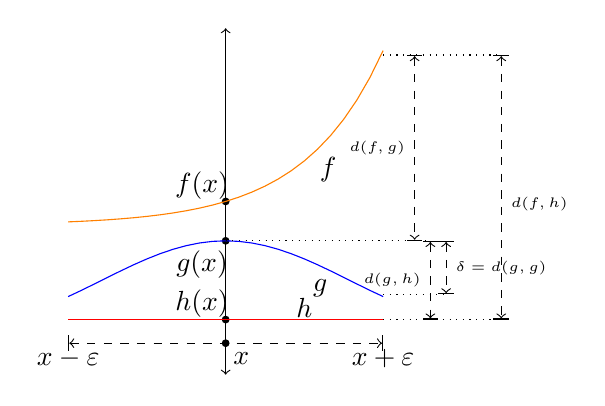
\begin{tikzpicture}[domain=-2:2]
%\draw[very thin,color=gray] (-0.1,-1.1) grid (3.9,3.9);
\draw[dashed, |<->|]   (-2,0) -- (2,0);
\draw[<->] (0,-0.4) -- (0,4); % node[above] {$f(x)$};

    \node at (0,0)[circle,fill,inner sep=1pt]{};
%    \node at (-2,0)[circle,fill,inner sep=1pt]{};
%    \node at (2,0)[circle,fill,inner sep=1pt]{};
\node(z) at (0.2,-0.2) {$x$};
\node(-e) at (-2,-0.2) {$x-\varepsilon$};
\node(e) at (2,-0.2) {$x+\varepsilon$};


\node(f) at (0,0.8+0.5)[circle,fill,inner sep=1pt]{};
\node(f) at (0,1.5+0.3)[circle,fill,inner sep=1pt]{};
\node(f) at (0,0.3)[circle,fill,inner sep=1pt]{};

\node(f) at (-0.3,2) {$f(x)$};

\node(f) at (-0.3,1) {$g(x)$};

\node(f) at (-0.3,0.5) {$h(x)$};

\node(ff) at (1.3,2.2) {{$f$}};
\node(gg) at (1.2,0.7) {{$g$}};
\node(gg) at (1,0.45) {{$h$}};

%\draw[color=red] plot (\x,\x) node[right] {$f(x) =x$};
% \x r means to convert ?\x? from degrees to _r_adians:
\draw[color=blue] plot (\x,{0.8+ 0.5*(cos(\x r))}) ;
\draw[color=orange] plot (\x,{1.5+0.3*exp(\x)}) ;
\draw[color=red] plot (\x,{0.3}) ;



\draw[dotted] (0,1.3) -- (2.6,1.3);
\draw[dotted] (2,0.3) -- (3.5,0.3);
\draw[dotted] (0,1.3) -- (2.4,1.3);
\draw[dotted] (2,3.66) -- (3.5,3.66);
\draw[dotted] (2,0.62) -- (2.8,0.62);

%
%\draw[dotted] (0,1.8) -- (2, 0.62);
%\draw[dotted] (0,1.3) -- (2, 3.66);

\draw[dashed,|<->| ] (2.4,3.66) -- node[left] {\tiny$d(f,g)$} (2.4,1.3);
\draw[dashed,|<->| ] (2.6,1.3) -- node[left] {\tiny$d(g,h)$} (2.6,0.3);

\draw[dashed,|<->| ] (2.8,1.3) -- node[right] {\tiny$\delta=d(g,g)$} (2.8,0.62);

%\draw[dashed,|<->| ] (3.5,2.96) -- node[above right] {\tiny$\begin{matrix}d(f,g)+d(g,h)\\ -d(g,g)\end{matrix}$} (3.5,0.3);

\draw[dashed,|<->| ] (3.5,3.66) -- node[below right] {\tiny$d(f,h)$} (3.5,0.3);

\end{tikzpicture}
}
%
\caption{\small The distance arising from differential logical relations is not a partial metric: the example above shows that $d(f,h)> d(f,g)+d(g,h)- d(g,g)$ (with all distances computed at $(x,\varepsilon)$).}% and 
%
%
%minimum $\delta$ such that for all $y\in [x-\varepsilon, x+\varepsilon]$, both $g(y)\in [f(x)-\delta, f(x)+\delta]$ and $f(y)\in[g(x)-\delta, g(x)+\delta]$ hold. $\delta$ is thus $\max\{\delta_{1},\delta_{2}\}$ in the image above.}
\label{fig:graph2}
\end{subfigure}
\caption{Differential logical relations do not yield partial metrics.}
\end{figure}

A primary source of inspiration for our approach was the recent work by Dal Lago, Gavazzo and Yoshimizu on  \emph{differential logical relations} \cite{dallago:differential-stlc}. This is a semantical framework for higher-order languages in which a type is interpreted as a set $X$ endowed with a kind of metric structure expressed by a ternary relation $\rho \subseteq X\times Q\times X$, where $Q$ is an arbitrary quantale. To our knowledge, this is the first place were the idea of varying the quantales in which distances are measured is introduced as a key ingredient to obtain a cartesian closed category.

While the relation $\rho$ of a GMS induces a distance function $d_{\rho}(x,y)=\sup\{\varepsilon\mid \rho(x,\varepsilon,y)\}$, this function is not a (partial) metric. We can show this fact with a simple example: in this model the distance between two programs 
 $f,g:\mathsf{Real}\to \mathsf{Real}$ is taken in the quantale of functions from $\R\times \R_{+}^{\infty}$ to $\R_{+}^{\infty}$: intuitively, 
  $d(f,g)$ associates a closed interval $[x-\varepsilon,x+\varepsilon]$ (corresponding to the pair $(x,\varepsilon)$) with the smallest distance $\delta$ such that $[ f(x)-\delta, f(x)+\delta]$ and $[g(x)-\delta,g(x)+\delta]$ both contain the images of $[x-\varepsilon, x+\varepsilon]$ through
 $g$ and $f$ respectively (see Fig. \ref{fig:graph1}). Then, as shown in Fig. \ref{fig:graph2}, by letting $\delta=d(g,g)(x,\varepsilon)$, we have that $d(g,g)$ sends the interval $I=[x-\varepsilon, x+\varepsilon]$ onto the interval $[g(x)-\delta, g(x)+\delta]$, which has diameter $2\delta$, while the image of $I$ has diameter $\delta$, making the triangular law of partial metrics fail. 


\subparagraph*{Diameter Space over a Cartesian Closed Category}

Our approach was devised primarily to account for transformations in higher-order languages designed for real analysis computation (like \emph{e.g.} $\mathsf{Real\ PCF}$ \cite{Edalat:2000aa}). However, diameter spaces can be constructed starting from any higher-order programming language with a reasonable denotational semantics. In fact, for \emph{any} cartesian closed category $\mathbb C$, we can construct a cartesian \emph{lax-}closed category $\dsp(\mathbb C)$, whose morphisms can be seen as approximate versions  of the morphisms of $\mathbb C$. The ``lax'' preservation of the cartesian closed structure reflects the fact that, by composing approximations in a higher-order setting, also their error rates compose (typically, approximating non $\beta$-normal $\lambda$-terms will lead to higher error-rates than approximating their $\beta$-normal forms). 



The generality of our construction shows in particular that our partial metric semantics requires no restrictions (\textit{e.g.} Lipschitz-continuity) on morphisms, and adapts well to the model one starts with: for instance, the category $\dsp(\set)$ contains a partial metric on the set of \emph{all}  set-theoretic functions from $\mathbb R$ to $\mathbb R$, while the categories $\dsp(\eff)$ (where $\eff$ is the \emph{effective topos} \cite{hyland:effective-topos}) and $\dsp(\scott)$ show that our approach scales well to a more computability-minded setting.

